\documentclass[11pt,a4paper]{article}
%\usepackage{fullpage}
\usepackage[total={6.5in,8.75in},
top=1.2in, left=0.9in]{geometry}
\usepackage[utf8]{inputenc}
\usepackage[english]{babel}
\usepackage{amsmath, amsthm}
\usepackage{amsfonts}
\usepackage{amssymb}
\usepackage{graphicx}
\usepackage{pifont}
%\usepackage{bussproofs}
\usepackage{enumitem}
\usepackage{centernot}
\usepackage{xspace}
\usepackage{stmaryrd}
\usepackage{mathtools}
\usepackage{cleveref}
\usepackage{listings}
\usepackage{tikz-qtree}
\usepackage{tikz}
\usepackage{algorithm}
\usepackage{algorithmicx}
\usepackage{algpseudocode}
\usepackage[hidelinks]{hyperref}
\usetikzlibrary{automata,trees,fit,backgrounds,shapes,snakes}
\usetikzlibrary{decorations.shapes}
\usepackage{float}
\usepackage{fancyvrb}
\usepackage{framed}
\usepackage{fancyhdr}
\usepackage{lastpage}
\usepackage{comment}

\usepackage[backend=bibtex,
%style=numeric,
style=alphabetic,
%style=reading,
sorting=ynt
]{biblatex}
\addbibresource{references}

\definecolor{light-gray}{gray}{0.95}
\newcommand {\conf} [1] {\ensuremath{\left\langle #1 \right\rangle}}
\newcommand {\bstep} {\ensuremath{\Downarrow}}
\newcommand {\bstepA} {\bstep_{ A}}
\newcommand {\bstepB} {\bstep_{ B}}
\newcommand {\bstepC} {\bstep_{ C}}
%\newcommand {\co} [1] {\ensuremath{\operatorname{\bf #1}}}
\newcommand {\coo} [1] {\ensuremath{\operatorname{\mathsf{#1}}}}
\newcommand {\co} [1] {\coo{#1}}
\newcommand {\pp}  {\ensuremath{\mbox{\footnotesize{++}}}}
\newcommand {\Skip} {\co{skip}}
\newcommand {\Not} {\co{not}}
\newcommand {\Iff}[3] {\co{if} (#1) \co{then} #2 \co{else} #3}
\newcommand {\Ifp}[3] {\co{ifp} (#1) \co{then} #2 \co{else} #3}
%\newcommand {\While}[2] {\co{while} #1 \co{do} #2}
%\newcommand {\Repeat}[2] {\co{repeat} #1 \co{do} #2}
\newcommand {\Input} {\co{input}}
%\newcommand {\Break} {\co{break}}
%\newcommand {\Continue} {\co{continue}}
\newcommand{\True}{\co{True}}
\newcommand{\False}{\co{False}}
\newcommand{\Or}{\co{or}}
\newcommand{\Let}[1]{\coo{let} #1 \coo{in} }
\newcommand{\Lam}{\ensuremath{{\lambda}}}
\newcommand{\Ref}{\coo{ref}}
\newcommand{\Int}{\coo{int}}
\newcommand{\bool}{\coo{bool}}
\newcommand{\Bool}{\bool}
\newcommand{\Unit}{\coo{unit}}
\newcommand{\Rec}[1]{\left\{#1\right\}}
\newcommand{\pa}[1]{\left(#1\right)}
\newcommand{\dt}[1]{\left|\arr{#1}\right|}
\newcommand{\ba}[1]{\left\langle #1\right\rangle}
\newcommand{\tree}{\coo{tree}}
\newcommand{\fa}{\coo{\forall}}
\newcommand{\more}[1]{\vdots\hspace{-1mm}~^{#1}}
\newcommand{\f}[1]{\textsc{#1}}
\newcommand{\g}[1]{\textsf{#1}}
\newcommand{\finite}{\co{finite}}
\newcommand{\lift}[1]{\left\lfloor #1 \right\rfloor}
\newcommand{\ttwo}{\mbox{\scriptsize\ding{173}}}

\newcommand{\trans}[2]{\ensuremath{\mathcal{#1}\left\llbracket #2\right\rrbracket}}

\newtheorem*{lemma}{Lemma}
\newtheorem*{theorem}{Theorem}
\newtheorem*{definition}{Definition}
\newtheorem*{corollary}{Corollary}

\lstset{ %
  language=Java,                % the language of the code
  basicstyle=\footnotesize,           % the size of the fonts that are used for the code
  numbers=left,                   % where to put the line-numbers
  numberstyle=\tiny\color{gray},  % the style that is used for the line-numbers
  stepnumber=1,                   % the step between two line-numbers. If it's 1, each line 
                                  % will be numbered
  numbersep=10pt,                  % how far the line-numbers are from the code
  backgroundcolor=\color{white},      % choose the background color. You must add \usepackage{color}
  showspaces=false,               % show spaces adding particular underscores
  showstringspaces=false,         % underline spaces within strings
  showtabs=false,                 % show tabs within strings adding particular underscores
  mathescape=true,
  frame=leftline,                   % adds a frame around the code
  rulecolor=\color{gray},        % if not set, the frame-color may be changed on line-breaks within not-black text (e.g. comments (green here))
  tabsize=2,                      % sets default tabsize to 2 spaces
  captionpos=t,                   % sets the caption-position to bottom
  breaklines=true,                % sets automatic line breaking
  breakatwhitespace=false,        % sets if automatic breaks should only happen at whitespace
  title=\lstname,                   % show the filename of files included with \lstinputlisting;
                                  % also try caption instead of title
  escapeinside={\%*}{*)},            % if you want to add LaTeX within your code
  morekeywords={*,...},              % if you want to add more keywords to the set
  deletekeywords={...}              % if you want to delete keywords from the given language
}

\newcommand\tmark[2]{%
  \ensuremath{\tikz[baseline] \node[anchor=base] (#1) {#2};}}
\tikzstyle{every picture}+=[remember picture]
\newcommand{\tm}[2]{\tmark{#1}{\ensuremath{#2}}}
\newcommand{\tr}[2]{\tmark{#1}{\color{red}{\ensuremath{#2}}}}
\newcommand{\arr}[1]{\begin{array}{cccccccccc} #1\end{array}}
\newcommand{\mat}[1]{\left(\arr{#1}\right)}
\newcommand{\Malloc}{\co{malloc}}
\newcommand{\Null}{\co{null}}

\newcommand{\SN}{\ensuremath{\mathcal{SN}}}
\newcommand{\Inl}{\co{inl}}
\newcommand{\Inr}{\co{inr}}
\newcommand{\Case}[3]{\co{case}~#1~\co{of} #2 \mid #3}
\newcommand{\R}{\co{rec}}
\newcommand{\Fold}{\co{fold}}
\newcommand{\Unfold}{\co{unfold}}
\newcommand{\coerce}[1]{\ensuremath{\Theta\left\llbracket #1\right\rrbracket}}

\allowdisplaybreaks

\usepackage{setspace}
\doublespacing

\setlength{\headheight}{15pt}
 
\pagestyle{fancyplain}
%\renewcommand{\chaptermark}[1]{\markboth{#1}{}}
 
\lhead{\fancyplain{}{\footnotesize\leftmark}}
\chead{}
\rhead{}
\lfoot{}
\cfoot{\thepage\ of \pageref{LastPage}}
\rfoot{}

\usepackage[protrusion=true,expansion=true]{microtype} % Better typography
\usepackage{graphicx} % Required for including pictures
\usepackage{wrapfig} % Allows in-line images

\author{Clifford Chou, Bryan Cuccioli, Lee Gao, 
Favian Contreras}
\date{\today}
\title{\textbf{Intermediate Progress Report}} % Subtitle

\begin{document}
\tikzset{every tree node/.style={minimum width=2em,draw,circle},
         blank/.style={draw=none},
         edge from parent/.style=
         {draw, edge from parent path={(\tikzparentnode) -- (\tikzchildnode)}},
         level distance=1.5cm}


\renewcommand{\abstractname}{Abstract} % Uncomment to change the name of the abstract to something else
\begin{singlespace}
\maketitle
\begin{abstract}
We explore what we believe to be a novel approximate measure in the 
``efficiency'' of large software engineering projects. Many software systems 
are so large and complex that it is impossible to reason about their
runtime properties using conventional techniques in runtime 
analysis. As such, an approximation of this property is often used, but even 
then, it is difficult to create heuristics to judge whether a system is 
efficient or not. Our approach treats the interaction between the different 
subroutines of a system as network behaviors and approximates the running time 
of a system by the most number of calls to a single function. Having 
experimentally determined that various large software systems behave like scale
-free networks, we gain an asymptotic characterization of the growth of the max
-degree node within the call-graph which lets us approximate that the running 
time of such systems with code size $n$ slows down according to 
$O(\sqrt[\alpha]{n})$ for some $1 < \alpha \le 2$.
\end{abstract}

\hspace*{3,6mm}\textit{Keywords:} {\sf \small  scale-free networks, software 
engineering, static analysis, linear interpolation} % Keywords
\end{singlespace}
\vspace{10pt} % Some vertical space between the abstract and first section

%\setlength{\parindent}{0pt}

\section*{Introduction}
One of the biggest problems in the software development world is trying to 
reason about the efficiency of the software systems that are being developed. 
Traditional runtime analysis techniques tend to focus on algorithms as 
individual components and are rarely amenable to large scale systems because 
of the inherent difficulty in exploring the relationship between large numbers of 
different components of the system. Therefore, there is demand to 
automatically analyze these systems.

Conventional techniques are rather cumbersome and require a lot of 
sophisticated machinery. Oftentimes, these techniques do not scale to large 
projects with complex interactions between their various subroutines. However, 
from experience, in profiling and optimizing code most of the 
benefits come from reducing either the code size or the complexity of 
functions that get called the most. As such, we devised a measure of the 
complexity of a project based on how many incoming function calls each 
function might receive. One motivation for this is that this measure 
essentially maps to the indegree $k_{max}$ parameter (the expected maximum 
degree of the nodes of a network) of a graph structure that models the calls-
into interaction between the various functions, which we will henceforth
refer to as a call-graph.

More formally, using a simplified model,  define a program $P$ as a 
collection of functions $\ba{\vec f}$ along with a main function 
$f^* \in \ba{\vec f}$ acting as the entry-point. Define the function 
$\f{calls-to}: \g{fun} \to \g{set}(\g{fun})$ that returns the set of functions 
that \textit{can}\footnote{This is a subtle notion, since the 
function $f \triangleq \lambda x: \Iff{1 = 2}{g(x)}{h(x)}$ \textbf{cannot} in 
actuality call $g$ because it's never the case that $1 = 2$, but since this 
happens so rarely in practice, we will say that $f$ can call $\Rec{g,h}$} be 
called. Furthermore, let's define a relation 
$\co{calls} \subseteq \g{fun} \times \g{fun}$ such that 
$$f \co{calls} g \iff g \in \f{calls-to}(f).$$
Define the call-graph induced by program $P$ to be 
$$G_P = \pa{\ba{\vec f}, \co{calls}}$$
such that the nodes of $G_P$ are the functions in the program and the edges 
are the pairs $(f,g) \in \co{calls}$\footnote{Recall notationally, 
$f\co{calls}g$ is equivalent to $(f,g) \in \co{calls}$} so that we connect an 
edge from $f$ to $g$ if $f$ can call $g$.

Because programming languages obey a very strict semantic model, we 
hypothesized that this likely means that there's some kind of preferential 
attachment to certain functions over others. As such, we believed that $G_P$ 
will be scale-free in the sense that\cite{DUR}
\begin{itemize}
\item the indegree distribution of the nodes of $G_P$ forms a power law 
distribution; suppose $p(k)$ is the probability that a vertex in $G_P$ has 
indegree $k$, then $p(k) \sim C k^{-\gamma}$ and
\item furthermore, $2 \le \gamma \le 3$.
\end{itemize}
It turns out that scale-free networks have various useful properties that we 
can exploit, one of which is the characterization of the expected maximum 
indegree of the graph $k_{max}$, which corresponds to the function in $G_P$ 
that gets \emph{called into} the most often. 
\section*{Characterizing $k_{max}$ for Scale-Free Networks}
Recall that the indegree distribution of a scale-free network has probability 
density function
$$
p(k) = C k^{-\gamma}
$$
where 
$$
C \sum_{k=0}^\infty k^{-\gamma} = 1 \implies 
C = \frac{1}{\sum\limits_{k=0}^\infty k^{-\gamma}} = \zeta(\gamma)^{-1}
$$
if we approximate $\sum \approx \int$, then
$$
\zeta(\gamma) \approx \int_1^\infty x^{-\gamma} dx = \pa{\gamma-1}^{-1}
$$
Now, suppose we want to find $k_{max}$, then in a discrete sense, we would 
expect that the probability of $p(k > k_{max})$ must be smaller than the 
probability to just pick one node out of all of the $n$ nodes, so that, 
working in the continuous approximation
$$
\int_{k_{max}}^\infty (\gamma -1)k^{-\gamma} dk = k_{max}^{1-\gamma} \approx 
\frac{1}{n}
$$
and so $k_{max} \approx \sqrt[\gamma - 1]{n}$. \cite{CLASS}

\section*{Static Analysis Framework}
In order to test our hypothesis, we first needed to create the tools required 
to construct $G_P$. We chose to analyze Java programs because of the large 
number of open source software in the wild that we can use as well as the 
existing support for doing these types of analysis on Java. 

Now, redistributed Java software is typically composed of a collection of 
compile \emph{bytecode} that can be executed by the Java Virtual Machine, 
which is part of the Java runtime environment. Because the bytecode language 
is much more structured and easier to analyze than the textual Java 
programming language itself, we chose to construct the call-graph of the 
translated bytecode (encapsulated in the \emph{.class} files). In order to 
parse and work with compiled code, we used the well-established OCW ASM2 
package. \cite{ocwasm} 

Since we only care about the invocation relationship between the different 
functions, the static analysis of the bytecode is not difficult.
\begin{algorithm}
\caption{Constructing the Call Graph}
\begin{algorithmic}
\Function{Analyze}{$P = \ba{\vec f}$}
\State $G_P \gets \g{new}~ \g{Graph}()$
\For{$\g{fun}~f \in P$}
\For{$\g{instruction}~i \in f.\g{instructions}$}
\If{$i$ is a method-call to $\g{fun}~g$}
\State Add edge $f \to g$ into $G_P$
\EndIf
\EndFor
\EndFor
\EndFunction
\end{algorithmic}
\end{algorithm}
After we've constructed $G_P$, we now need to construct the indegree frequency 
of $G_P$, which in essence counts the number of edges coming into each 
function in $G_P$. We decide to represent this abstract notion of a frequency 
table as a concrete mapping $\f{FreqIn}: \g{fun} \to \mathbb{N}$ within our 
analysis. We then computed the distribution of the degrees also concretely as 
a mapping $\f{Dist}: \mathbb{N} \to \mathbb{N}$ which maps each positive 
degree to the number of nodes of such degree there are within $G_P$.
\begin{figure}
\centering
\caption{}
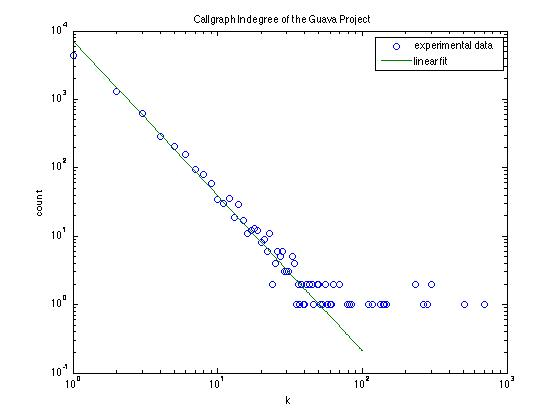
\includegraphics[scale=0.6]{dist}
\end{figure}
\section*{Assessing Goodness of Fit and Linear Interpolation}
We analyzed the source code two large open source Java projects (Guava and 
OCW's ASM project) and found that the degree distribution follows a
power law based on their \g{loglog} plots. Recall that if a distribution has
density $p(k) \sim Ck^{-\gamma}$, then $\log(p(k)) = \log(C) - \gamma \log(k)$
so its distribution density should look roughly linear.

In order to determine the power law coefficient $\gamma$, we resort to linear
algebra. We are give a list of degrees $k$ and a list of frequencies of these 
degrees $y$, and we want to find the parameters $C,\gamma$ so that 
$\hat y(k) = Ck^{-\gamma}$ best fits the observed data. Since non-linear 
interpolation is a hard problem, we can transform the data logarithmically into
a linear interpolation problem
$$
\arg\min_{C,\gamma} \|(\log(C) - \gamma \log(k)) - \log(y)\|_2^2.
$$
A monotonicity argument with respect to $\log$ should guarantee that the
minimum of this system is also optimal when we transform this instance back
via $\exp$.

Now, let $\bar k = \log k, \bar y = \log y, \bar C = \log C$, let $n = \g{length}(k)$
 and let $A$ be the $n \times 2$ matrix 
 $$\small A = \mat{1 & \bar k_1 \\ 1 & \bar k_2 \\ \vdots \\ 1 & \bar k_n}$$ 
then we are attempting to find the solution $x = \pa{\bar C, -\gamma}^T$ such 
that $\min_x \|Ax - \bar y\|$ is minimized. We can solve this via the normal equation 
\cite{linalg} so that  $x = (A^TA)^{-1}A^T\bar y$. Since this is just a 2 by 2 system
$$
x = \mat{n & \sum_i \bar k_i \\ \sum_i \bar k_i & \bar k^T\bar k}^{-1} 
\mat{\sum_i \bar y_i \\ \bar k^T\bar y} 
= \frac{1}{n\cdot \bar k^T\bar k - \pa{\sum \bar k}^2} 
\mat{\bar k^T \bar k \cdot \sum \bar y - \sum_i \bar k \cdot \bar k^T\bar y \\ 
n \bar k^T \bar y - \pa{\sum_i \bar k}\pa{\sum_i \bar y}}
$$
so we know that $\gamma = 
\frac{\pa{\sum_i \bar k}\pa{\sum_i \bar y}- 
n \bar k^T \bar y}{n\cdot \bar k^T\bar k - \pa{\sum \bar k}^2}$ which is easily
computable. 

In the case of the Guava project, the distribution has coefficient $\gamma = 2.27$
which suggests that it is within the realm of a scale-free network \cite{CLASS}, 
as can be seen in 
figure 1. However, we see that since we have a discrete distribution, it is impossible
for the pattern to carry one once $p(k) < 1$ since we cannot have fractional counts,
therefore we develop a rather interesting phenomenon of a fat tail distribution.
When left untreated, this will tend to skew our distribution.

\section*{Moving Forward}
There are many things left to do that we will still need to implement. 
\begin{enumerate}
\item 
First and 
foremost, in order to be objective, we will need to evaluate many more projects to
determine whether this scale-freeness is a property of just the small sample that 
we've currently tested or it is more likely that this is a global phenomenon.
\item 
Secondly, it has come to our attention that many of these scale-free distributions
are actually exponentially damped. Therefore, it is worthwhile to explore whether
our model may improve with various "extensional" distributions.
\item 
There's also the issue that automatic analysis to infer the exponent on the coefficient
is difficult right now because the fat tail is fudging the result. After a little bit of 
thought and some consultation with existing research, we realized that if $p(k = x)$ 
is power law, then so too is the cumulative density $p(k \ge x)$ as long as 
$\gamma > 1$. In fact, it can be shown that \cite{CLASS}
$$
p(k \ge x) = \zeta(\gamma) x^{1-\gamma}
$$
this is great because we can instead compute the cumulative degree distribution 
density, which is not effected by the fat tail (which have low frequencies that are 
almost negligible after accumulating all of the degree counts together). Since this 
too is a power law, we can use the same exact technique as before to get the 
parameter $\alpha = \gamma-1$ and set $\gamma = \alpha + 1$.
\item 
Discover a concrete application of this analysis. Right now, this analysis affords us 
with the knowledge that the function that ``gets called most often'' should get 
called more often at the rate of $O(\sqrt[\gamma-1]{n})$ for $n$ some measure of
the size of the program. We can likely use this as a crude estimator on whether 
implementing certain optimizations on the program is worth the effort, and to 
predict at what point in the future we will need to do significant rewrite of the
program in order to improve efficiency.
\end{enumerate}
\medskip

\printbibliography[title={References}]

\end{document}
